%version of 03-17-20

\chapter{The Vertigo of Infinity:
Handling the Very Large and the Infinite}
\label{ch:infinity}

\begin{quote}
{\em One Two Three \ldots Infinity} \\
\hspace*{1in}George Gamow, 1947 book
\end{quote}

\medskip

\noindent
An immensely powerful attribute of the way mathematics allows us to deal with quantity is our ability---in principle, at least---to use identical reasoning and tools of analysis to manipulate all finite objects: We do not need---to cite just two examples---a hierarchy of arithmetics to deal with real numbers of various sizes nor a variety of logical calculi to deal with propositions having various numbers of satisfying assignments of truth values.  This situation changes, however, when we deal with objects---say, sets or numbers---whose sizes can change {\em dynamically} or that are composed of {\em infinitely many} distinguishable objects.  In order to reason rigorously about quantities that can grow---or, equivalently, can shrink---without bound, we need new conceptual machinery.  This is true whether or not the growth can continue forever!  And, we need yet other new conceptual tools to deal with objects that are actually infinite.

\smallskip

This chapter is devoted to developing the needed tools and to heightening readers' awareness of the care that they must take when reasoning in the domain of this chapter's title: the {\em large}, the {\em very large}, and the {\em Infinite}.

\section{Asymptotics}
\label{sec:asymptotics}

\index{asymptotics}
{\em Asymptotics} can be viewed as a language and a system of reasoning that allow one to talk in a {\em qualitative} voice about {\em quantitative} topics.  We thereby generalize to arbitrary growth functions terms such as ``linear'', ``quadratic'', ``exponential'', and ``logarithmic''.

Such a language and system are indispensable if one needs to reason about computational topics over a range of situations, such as a range (``all existing''?)~of computer architectures and software systems.  As two simple examples: (1) Carry-ripple adders perform additions in a number of steps that is linear in the lengths $n$ of the summands (measured in number of bits)---no matter what these lengths are.  (2) Comparison-based sorting algorithms can sort lists of $n$ keys in a number of steps proportional to $n \log n$, but no faster---where the base of the logarithm depends on the characteristics of the computing platform and the set of keys being sorted.  More precise versions of the preceding statements require specification of the number $n$ and other details, possibly down to the clock speeds of the host computer's circuitry.

\smallskip

The need for the material in this section can be discerned (almost) daily, as the news media report---and all too often {\em misreport}---about dynamic quantities: the word ``exponential'' is
very often used when ``fast'' or ``large" is what is actually meant.  It is not true (usually) that ``Country A's GDP'' or ``The X-virus epidemic'' is growing {\em exponentially}.  Country B's strategic planning, in the first example, and the government's public health department, in the second example, cannot proceed rationally without trustworthy quantitative information.

\subsection{The Language of Asymptotics}
\label{sec:language-asymptotics}

The language of asymptotics has its origins in the subfield of mathematics known as {\it Number Theory}, in the late 19th century.  The basic version of the language---which handles almost all situations one encounters when studying the discrete mathematics germane to computational phenomena---builds on the terminology we discuss here.  There is an advanced companion to the following notions, which builds on nondiscrete concepts such as limits; this advanced material will be beyond the likely needs of most students of computing---excepting, of course, specialists in specific, advanced subject areas.  The basics of the language of asymptotics build on three primitive notations and notions.  We need only the rudiments of this material within this text, so we refer the reader to standard texts on algorithm design and analysis (e.g.,\cite{CLRS}) or number theory (e.g., \cite{NivenZ80}), to go beyond the basics of the following ideas.

\smallskip

The following notation actually has several variants in both symbology and articulation.  We elaborate on this situation only for our first notation, the ``big-$O$'' (articulated ``big $O$").  The reader should be aware that analogous complications accompany our other two notations, the ``big-$\Omega$'' (articulated ``big Omega") and the ``big-$\Theta$'' (articulated ``big Theta"). 
\index{big-$O$}\index{big-$\Omega$}\index{big-$\Theta$} \index{asymptotic notation}
\begin{itemize}
\item
{\em The big-$O$ notation}.
The assertion $f(x) = O(f_1(x))$ says, intuitively, that the function $f$ {\em grows no faster than} the function $f_1$.  It is, thus, the asymptotic analogue of ``less than''.

\smallskip

Formally, the assertion

\hspace*{.2in}$f(x) = O(f_1(x))$

means

\hspace*{.2in}
$(\exists c >0)(\exists x_1)(\forall x > x_1)
[f(x) \leq c \cdot f_1(x)]$

\medskip

\noindent \fbox{
\begin{minipage}{0.96\textwidth}
{\bf Explanatory note}.

{\it The complication}.

The ``equal sign'' in the notation $f(x) = O(f_1(x))$ does {\em not} mean ``equals''.

\smallskip

In fact, the assertion ``$fx) = O(f_1(x))$'' actually means that function $f$ {\em belongs to the class of functions that {\em eventually} grow no faster than function $f_1$ does.}

\smallskip

Consequently:
\begin{enumerate}
\item
The assertion ``$f(x) = O(f_1(x))$'' is {\em articulated}

\smallskip

\hspace*{.25in}``$f(x)$ {\em is} $O(f_1(x))$''.

\smallskip

{\em Never} substitute ``equals'' for ``is''
\item
Many people acknowledge the ``belonging to a class'' facet of the definition by writing

\smallskip

\hspace*{.25in}``$f(x) \in O(f_1(x))$''

\smallskip

rather than

\smallskip

\hspace*{.25in}``$f(x) =  O(f_1(x))$''
\end{enumerate}

\medskip

{\it An esoteric aside}:  It is strange that precisely two of the three asymptotic letters, namely, $\Omega$ and $\Theta$, come from the Greek alphabet.  In fact, many scholars insist that the letter $O$ in ``big-$O$" is actually the Greek letter omicron, {\em not} the Latin letter $O$.
\end{minipage}
}
\bigskip

\item
{\em The big-$\Omega$ notation}.
The assertion $f(x) = \Omega(f_2(x))$ says, intuitively, that the function $f$ {\em grows at least as fast as} function $f_2$.  It is, thus, the asymptotic analogue of ``greater than''.

\smallskip

Formally, the assertion

\smallskip

\hspace*{.2in}
$f(x) = \Omega(f_2(x))$

means

\hspace*{.2in}
$(\exists c >0)(\exists x_2)(\forall x > x_2)
[f(x) \geq c \cdot  f_2(x)]$

\item
{\em The big-$\Theta$ notation}.
The assertion $f(n) = \Theta(f_3(n))$ says, intuitively, that the function $f$ {\em grows at the same rate as} function $f_3$.  It is, thus, the asymptotic analogue of ``equal to''.

\smallskip

Formally, the assertion

\smallskip

\hspace*{.2in}
$f(x) = \Theta(f_3(x))$

means

\hspace*{.2in}
$(\exists c >0)(\exists c' >0)(\exists x_{3})(\forall x > x_{3})
[c \cdot f_3(x) \leq f(x) \leq c' \cdot  f_3(x)]$
\end{itemize}
One renders the preceding intuitive explanations precise by pointing out that the three specified relations:
\begin{enumerate}
\item
take hold {\em eventually}, i.e., only for large arguments to the functions $f$, $f_1$, $f_2$, $f_3$;
\item
hold only up to an unspecified constant of proportionality.
\end{enumerate}
The plots in Fig.~\ref{fig:Asymptotic} illustrate the definitions of big-$O$ and big-$\Omega$ graphically.
\begin{figure}[htb]
\begin{center}
       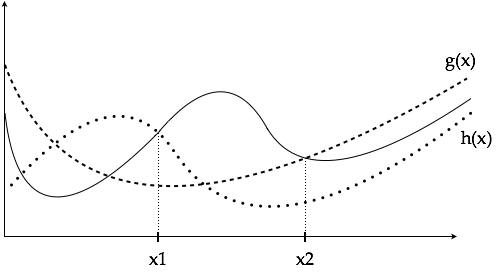
\includegraphics[scale=0.4]{FiguresArithmetic/NotationAsymptotic}
\caption{Plots of three functions: $f$ (solid curve), $f_1$ (dotted curve that originates on the left, above $f$), and $f_2$ (dotted curve that originates on the left, below $f$).  Assume that the three illustrated trajectories continue in the depicted relationships for large values of $x$---i.e., for all $x > x_1$, the plot for $f$ lies strictly below that for $f_1$ and strictly above that for $f_2$.  With this assumption, the figure illustrates the relations: $f(x) = O(f_1(x))$ and $f(x) = \Omega(f_2(x))$.}
\label{fig:Asymptotic}
\end{center}
\end{figure}

\subsection{The ``Uncertainties'' in Asymptotic Relationships}
\label{sec:uncertainties-asymptotics}

The formal definitions of all three of our asymptotic relationships are bracketed by two important quantifiers:
\[ 
(\exists c >0) \ \ \ \mbox{ and }  \ \ \  (\forall x > x^{\#}).
\]
The former, {\em uncertain-size} quantifier ($\exists c >0$), asserts that asymptotic notions describe functional behavior ``in the large''.  Thus, in common with more common qualitative descriptors of quantitative growth such as ``linear", ``quadratic", ``cubic", ``quartic", ``exponential", ``logarithmic", etc., asymptotic relationships give no information about constants of proportionality.  {\em We are not saying that constant factors do not matter!}  We are, rather, saying, {\em We sometimes want to discuss growth patterns \underline{in the large} rather than in detail.}

\smallskip

The latter, {\em uncertain-time} quantifier ($\forall x > x^{\#}$) asserts that asymptotic relationships between functions are promised to hold only ``eventually'', i.e., ``for sufficiently large values of the argument $x$''.  Therefore:  {\em Asymptotic notions cannot be employed to discuss or analyze quantities that can never grow beyond a fixed finite value}.  The fact that all instances of a quantity throughout history have been below $N$ is immaterial, as long as it is conceivable that an instance larger than $N$ could appear at some time in the future.

\smallskip

These two quantifiers in particular distinguish claims of asymptotic relationship from the more familiar definite inequalities such as
\[ [f(x) \leq g(x)] \ \ \ \ \mbox{ or } \ \ \ \ [f(x) \geq 7 \cdot g(x)] \]
In fact, it is often easier to think about our three asymptotic bounding assertions as establishing {\em envelopes} for $f(x)$---cf., Fig.~\ref{fig:Asymptotic}:
\begin{itemize}
\item
$f(x) = O(g(x))$.

If one draws the graphs of the functions $f(x)$ and $c \cdot g(x)$, then as one traces the graphs with increasing values of $x$, one eventually reaches a point $x^{\#}$ beyond which the graph of $f(x)$ never enters the territory {\em above} the graph of $c \cdot g(x)$.
\item
$f(x) = \Omega(g(x))$.

This situation is the up-down mirror image of the preceding one: just replace the highlighted ``{\em above}'' with ``{\em below}.''
\item
$f(x) = \Theta(g(x))$.

This relation provides a {\em two-sided} envelope:  Beyond $x^{\#}$, the graph of $f(x)$ never enters the territory {\em above} the graph of $c \cdot g(x)$ and never enters the territory
{\em below} the graph of $c' \cdot g(x)$.
\end{itemize}
In addition to allowing one to make familiar growth-rate comparisons such as ``$n^{14} = O(n^{15})$'' and ``$1.001^n = \Omega(n^{1000})$,'' we can now also make assertions such as ``$\sin x = \Theta(1)$,'' which are much clumsier to explain in words.

\medskip

\index{asymptotics!with little letters}
\noindent {\bf Beyond the big letters.}
There are ``little''-letter analogues of the preceding ``big''-letter asymptotic relations and notations: $o$, $\omega$, and $\theta$.  The definitions and domains of application of these notations build on the notion of {\it limit}, which is fundamental in continuous mathematics---e.g., in the differential and integral calculus---but rare in discrete mathematics.  We therefore do not include this topic in this text, instead referring the reader to any good text on the calculus.

\subsection{Inescapable Complications}
\label{sec:asymptotic-complication}

The story we have told thus far is more or less standard fare in courses on discrete mathematics and algorithms.  Two complications to the story are covered less consistently, despite the fact that, lacking them, one cannot perform cogent asymptotic reasoning about modern computing
environments.  Both complications involve the notion of {\em uniformity}. 
\index{relations!uniformity}

\medskip

\index{asymptotics!multiple functions}
\noindent
{\bf 1.}
{\em Multiple functions}.
Say that we have four functions, $f, g, h, k$, and we know that
\[ f(n) = O(g(n)) \ \ \ \  \mbox{ and } \ \ \ \ h(n) = O(k(n)) \]
It is compellingly suggestive that
\[ f(n) + h(n) = O(g(n) + k(n)) \]
--- but is it true?

\smallskip

In short, the answer is {\em YES}---but verifying the answer requires a bit of subtlety.  The challenge is that, absent hitherto undisclosed information, the proportionality constants $c_{f,g}$ and $N_{f,g}$ that witness the big-$O$ relationship between functions $f$ and $g$ have no connection with the constants, $c_{h,k}$ and $N_{h,k}$ that witness the analogous relationship between functions $h$ and $k$.  Therefore, in order to verify the posited relationship between functions $f + h$ and $g + k$, one much find witnessing constants $c_{f+h, g+k}$ and $N_{f+h,g+k}$.

\smallskip

\noindent
Of course, this task requires only elementary reasoning---{\em but it must be done}!

\medskip

\index{asymptotics!multivariate functions}
\noindent {\bf 2.}
{\em Multivariate functions}.
Finally, we discuss the scenario that almost automatically accompanies the transition from {\em sequential, single-agent} computing to {\em parallel and/or distributed and/or multi-agent}computing.  One must account for a system's many resources: computing, memory/storage, and communication., etc.  One must assess the relationships among the costs of operating the system: time, energy, memory usage, etc.  One must account for possible tradeoffs among costs and possible cost-altering emulations of one subsystem by another. Within such scenarios, every assertion of an asymptotic relationship, of the form
\[ f(\vec{m}; \vec{n}) = O(g(\vec{m}; \vec{n})) \]
must explicitly specify the following information:
\begin{itemize}
\item
which variables represent resources that can grow without bound;
\item
among such unbounded variables, which participate in the posited asymptotic relation;
\item
for each participating unbounded variable $x$, what are the constants $c_x$ and $N_x$ that witness the posited asymptotic relationship(s).
\end{itemize}

\medskip

Clearly the complexity of cogent asymptotic reasoning---hence, also, the complexity of teaching about such reasoning---gets much more complicated in the multivariate settings engendered by parallel and distributed computing.  But, the benefits of being able to reason qualitatively about the quantitative aspects of computing increase at least commensurately!

\section{Reasoning about Infinity}
\label{sec:reasoning-infinity}

\subsection{Coping with infinity}
\label{sec:coping-infinity}

A recurring challenge when one ``does'' mathematics is dealing with {\em infinity}.  Infinite objects, such as sets and summations, behave rather differently from the more familiar finite objects that we encounter in our daily lives.  Two examples will suffice.  
\begin{enumerate}
\item
There are ``equally many'' integers within the set $\N$ of {\em all} integers as there are in
  \begin{itemize}
  \item
$\N$'s proper {\em subset} that comprises just the {\em odd} integers.
  \item
$\N$'s proper {\em superset} that comprises ordered pairs of integers.
  \end{itemize}
Does this mean that ``infinite is infinite", i.e., that one can match up the elements of any two infinite sets.
  
\smallskip

\noindent
{\em Decidedly NOT!}

\smallskip

\noindent
Alas!  We have to await Section~\ref{sec:FNS-uncountable} before we make the acquaintance of infinite sets that are ``bigger" than $\N$.  We shall appreciate this introduction all the more after Section~\ref{sec:pairing}, where we shall encounter a lot of infinite sets that ``should be bigger" than $\N$---but are not! 


\item
We have seen in Chapter~\ref{ch:Summation} that there exist summations of infinitely many positive numbers whose sum is finite (in the sense that the series {\em converges}).  The series
\[ 1 \ + \ {1 \over 2} \ + \ {1 \over 2^2} \ + \cdots + \ {1 \over 2^k} \ + \cdots \ \ = \ \ 2 \]
provides an example.

\smallskip

But, there exist other infinite summations whose ``sum is infinite'' (in the sense that the series {\em diverges}).  The {\it harmonic} series
\[ 1 \ + \ {1 \over 2} \ + \ {1 \over 3} \ + \cdots + \ {1 \over k} \ + \cdots \]
provides an example.
\end{enumerate}
There are clearly nonobvious concepts within the world of the infinite, which distinguish those infinite objects that behave more or less as we would expect from those infinite objects that don't.

\medskip

\index{paradox}
The world of the infinite is even more subtle than the preceding examples suggest.  This world hosts myriad {\em paradoxes}---situations that, in the words of the {\it New Oxford Dictionary}, ``combine contradictory features or qualities".\footnote{In detail, the {\it New Oxford Dictionary} defines a ``paradox'' as \\
``a statement or proposition that, despite sound (or apparently sound) reasoning from acceptable premises, leads to a conclusion that seems senseless, logically unacceptable, or self-contradictory''.}

\medskip

The remainder of this section is devoted to discussing and explaining the sometimes-confusing but always-fascinating world of the infinite.

\subsection{The ``Point at Infinity''}
\label{sec:point-at-infinity}

\index{limit} \index{continuity} \index{Riemann sphere} \index{Riemann, Bernhard}
In many situations, the difficulties encountered when dealing with infinite objects result from the conceptual fiction that there is, in fact, a ``point at infinity''---i.e., that one can treat infinity as just
another number.  In many mathematical environments, this fiction is an aid to reasoning which can be handled with totally rigor---but often only when accompanied by rather sophisticated mathematical machinery.  Two familiar examples of such mathematical machinery are the notions
of  {\it limit} and {\it continuity} (of a function).  A more advanced example of such machinery is the {\it Riemann sphere}, an invention of the 19th-century German mathematician Bernhard Riemann, which allows one to reason about the infinite two-dimensional plane by ``conformally'' wrapping the plane into a sphere whose ``south pole'' represents the zero-point (i.e., the origin) of the plane and whose ``north pole'' represents the ``point at infinity.''  There are many other, less-familiar, examples of such mathematical machinery, including advanced topics such as {\it types} in the domain of mathematical logic.

\medskip

Of course, we have already had some success in dealing with a quite sophisticated genre of infinite object:  In Chapter~\ref{ch:Summation}, we summed and manipulated a broad variety of infinite summations.  We are close to having the tools necessary to deal with a variety of other infinite objects; to cite just two:
\begin{enumerate}
\item
In Section~\ref{sec:pairing}, we shall demonstrate how to establish one-to-one correspondences between certain infinite sets, including, notably, any two of: the set $\N$ of integers, the set $\Q$ of rationals, and the set $\N \times \N$ of ordered pairs of integers.

\item
In Section~\ref{sec:FNS-uncountable}, we shall demonstrate that one {\em cannot} establish a one-to-one correspondence between the set $\N$ of integers and the set $\R$ of real numbers.
\end{enumerate}

\smallskip

The lesson of the preceding paragraphs is that there is no need to avoid dealing with infinity and its related notions---as long as one has the mathematical machinery necessary to: ($a$) define all needed notions unambiguously; ($b$) obtain well-defined results from all required operations and manipulations; ($c$) reason cogently about all the concepts and processes one employs.  That said, the scenarios described in the coming two subsections warn us to treat all aspects of infinity with care and respect.  The subsections point out two challenges often encountered when one reasons about the infinite.  Both challenges leave us with some form of {\em paradox}.

\subsubsection{Underspecified problems}
\label{sec:underspecified}

The paradoxes we present in this section require refined groundrules for their resolution.  The underlying problems {\em seem} to be totally specified---until one tries to develop their solutions.

\paragraph{A. Summing ambiguous infinite summations}

The first question we tackle was the subject of much concern as the topic of infinite summations emerged from its infancy in the 18th century.  The overriding question is, What can one learn from an infinite series that does not have a unique sum?  Much valuable work has been done on this question, most of which is beyond the scope of this text.  But the conundrum presented by 
such summations is valuable to consider.

\medskip

For our first source of puzzlement, we invoke the following infinite summation.
\[ S \ = \ 1 \ - \ 1 \ + \ 1 \ - \ 1 \ + 1 \ - \ 1 \ + \cdots \]
There are many conflicting, but well-reasoned, answers to questions about $S$:
\begin{itemize}
\item
{\it Does summation $S$ have a finite sum?} 
\item
If so: {\it Is this sum positive or negative?}
\end{itemize}

\smallskip

\noindent
Here are four plausible answers to these questions; you may find others.  The final answer, in particular, merits strong consideration.
\begin{enumerate}
\item
YES: $S \ = \ 0$

\smallskip

This response is justified by the following association of terms in summation $S$.
\begin{figure}[h]
\begin{center}
        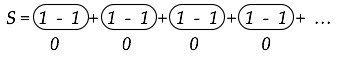
\includegraphics[scale=0.45]{FiguresArithmetic/InfiniteParadox1}
\end{center}
\end{figure}

\item
YES: $S \ = \ 1$

\smallskip

This response is justified by the following association of terms in summation $S$.
\begin{figure}[h]
\begin{center}
        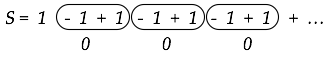
\includegraphics[scale=0.45]{FiguresArithmetic/InfiniteParadox2}
\end{center}
\end{figure}

\item
YES: $S \ = \ {1 \over 2}$

\smallskip

This response is justified by the fact that $S$ satisfies the equation $S \ = \ 1-S$.

\item
THERE IS NO VALID ANSWER.

\smallskip

This response is justified by the fact that the problem statement does not specify how to associate the terms of $S$.  As the first three answers suggest, ``mischievously" playing with parentheses enables us to arrive at many ``plausible'' sums for $S$.
\end{enumerate}

\medskip

The mysteries that arise from contemplating summation $S$ are not exhausted by playing with parentheses.  Consider the infinite summations consisting, respectively, of all odd integers, all even integers, and all integers:
\begin{eqnarray*}
S'  & = & 1 \ + \ 3 \ + \ 5 \ + \ 7 \ + \ 9 \ + \cdots \\
S'' & = & 2 \ + \ 4 \ + \ 6 \ + \ 8 \ + \ 10 \ + \cdots \\
S''' & = & 1 \ + \ 2 \ + \ 3 \ + \ 4 \ + \ 5 \ + \cdots
\end{eqnarray*}

All three of these summations must be ``positive''---whatever that term means in relation to infinite sums---because each is a sum of positive terms.  However, if one subtracts $S'$ from $S''$, one filters out the odd integers, which leaves us with the sum
\[ S''' \ - \ S' \ = \ S'' \ = \ 2 \times S''' \]
This result by itself is bizarre---we eliminate every other term and thereby double the sum!!  But one further step leaves us with the truly phantasmagorical expression
\[ S''' \ = \ - S' \]
which asserts the equality of a summation consisting of all positive numbers and a summation consisting of all negative numbers!

\ignore{***********
\begin{eqnarray*}
S' & = & 1 \ - \ 2 \ + \ 3 \ - \ 4 \ + \ 5 \ - \cdots + \cdots \\
S" & = & 1 \ + \ 3 \ + \ 5 \ + \ 7 \ + \ 9 \ + \cdots \\
S"' & = & 1 \ + \ 2 \ + \ 3 \ + \ 4 \ + \ 5 \ + \cdots
\end{eqnarray*}

\begin{itemize}
\item
One can argue that $S' \ = \ \frac{1}{4}$.

\smallskip

This conclusion derives from the valuation $S = {1 \over 2}$, in the light of the equation 
\[ S'  \ = \  S  \ - \ S'  \]

\item 
One can argue that $S" \ = \  \frac{1}{12}$.

\smallskip

This conclusion derives from the equation
\[ S" \ + \ S' \ =  1 \ + \ 4 \ + \ 8 \ + \ 12 \ + \ 16 \ + \cdots \ = \ 1 \ + \ 4 S" \]

 (hint: compute $C-B = 4+8+12+16+ \ldots$)
\end{itemize}
*******************}

\medskip

The preceding examples illustrate how very differently summations having infinitely many terms behave from summations having finitely many terms.

\medskip

{\em Beware:  Infinity is not a number!}

\paragraph{B. The Ross-Littlewood paradox}

\index{Littlewood, John E.} \index{Ross, Sheldon M.} 
\index{paradox!Ross-Littlewood paradox}
The following story is known as the {\it Ross-Littlewood paradox}, after its creators.  A version of the story appeared first in John Littlewood's enlightening and entertaining book {\it Littlewood's Miscellany} \cite{Littlewood-misc}; the story was amplified to its present form by Sheldon M.~Ross \cite{Ross76}. 

\medskip

Let us imagine a system that contains
\begin{itemize}
\item
a {\em really big} bin (in fact, one whose capacity grows as the story progresses)
\item
an unbounded sequence of ordered balls, labelled 1, 2, \ldots
\item
a {\em very} (read: infinitely) precise clock.
\end{itemize}
The system is watched over by a {\it Keeper}.  We observe the {\it Keeper} executing the following process.

\smallskip

\noindent {\sf Step $1$}.
At time {\em midnight minus $1$ minute}, the {\it Keeper} places the first ten balls in the sequence (i.e., balls $\#1, \ldots, \#10$) into the bin, and {\em immediately} removes the first ball (ball \#$1$).

\smallskip

\noindent {\sf Step $2$}.
At time {\em midnight minus $1/2$ minute}, the {\it Keeper} places the next ten balls in the sequence
(i.e., balls $\#11, \ldots, \#20$) into the bin, and {\em immediately} removes the second ball (ball \#$2$).

\smallskip

\noindent
The {\it Keeper} repeats this process endlessly, at midnight minus $1/4$ minute (putting balls $\#21, \ldots, \#30$ into the bin and removing ball \#$3$), then at midnight minus $1/8$ minute (putting
balls $\#31, \ldots, \#40$ into the bin and removing ball \#$4$), and so on.

\smallskip

\noindent
{\bf Question}: {\it How many balls are present in the bin at midnight?}  \\
(Note that ``infinity'' now measures the number of steps executed in the process.)

\medskip

\noindent
As in paragraph {\small\sf A}, there are several plausible answers to this question.  We provide just three.
\begin{enumerate}
\item
THERE ARE INFINITELY MANY BALLS.

\smallskip

This response is justified by the following reasoning.  Each step of the process inserts $10$ balls into the bin but removes only $1$ ball.  Hence, the population of the bin grows by $9$ balls after each step of the process---and it never decreases!  It follows, therefore, that after infinitely many steps, the bin's population must be infinite.

\item
THE BIN IS EMPTY---THERE ARE $0$ BALLS!

\smallskip

This response is justified by the following reasoning.  Every ball is eventually removed from the bin at some (finite) step of the process. Specifically, ball \#$n$ is removed at step $n$, i.e., at time midnight minus $2^{-n}$ seconds.

\item
THERE IS NO VALID ANSWER.

\smallskip

This response is justified by the following reasoning.  There is no ``moment at infinity'' that is actually ever encountered during the process.  That ``moment" is just a conceptual idealization.

\smallskip

In other words, infinity is not a number!
\end{enumerate}


\paragraph{C.  Zeno's paradox: Achilles and the tortoise}

\index{Zeno of Elea} \index{Zeno!Zeno's paradox} \index{paradox!Zeno's paradox}
In his celebrated {\it Paradox of Achilles and the Tortoise}, Zeno of Elea  presented a problem whose solution had to await the 17th century.

\smallskip

In Zeno's story, the slow-footed Tortoise (T) tries to convince the speedy Achilles (A) of the futility of trying to win any race in which A gives T even the smallest head start.  As long as T is ahead of A, says T, every time A traverses half the distance between himself and T, T will respond by moving a bit further ahead.  Thereby, T will always be a positive distance ahead of A, so that A can {\em never} catch T.

\smallskip

\index{infinitesimals}
At first glance, this story seems to call into question the physical reality of all motion.  In fact, the
resolution of the apparent paradox resides in the notion of {\em infinitesimals}---quantities that dynamically grow smaller than any finite number.  While infinitesimals are familiar today to anyone who has studied subjects such as the differential calculus, the notion of infinitesimal actually dates back only a few hundred years, to the 17th century.  

\medskip

\index{Leibniz (Leibnitz), Gottfried Wilhelm}  \index{Newton, Isaac} \index{Kronecker, Leopold} 

Underlying the discovery/invention\footnote{Were infinitesimals {\em discovered} or {\em invented}?  As you ponder this choice, recall the words of Leopold Kronecker that end our {\it MANIFESTO}.}~of infinitesimals is one of the great real-life mysteries of all time.  Who invented/discovered infinitesimals?  The parties to this dispute were the German mathematician Gottfried Leibniz \cite{Leibniz} and the English polymath (Sir) Isaac Newton \cite{Newton}.   The cases favoring each of these great men contain enough merit to guarantee that the dispute will likely never be settled.  We therefore list Leibniz and Newton alphabetically and give a coarse dating of the 17th century for the discovery.  This real-life mystery is as full of intrigue and suspense as any that one encounters in fiction.


\paragraph{D. Hilbert's hotel paradox}

\index{paradox!Hilbert's paradox}
While the final story of this section does not describe an actual paradox, it is often referred to by that term.  Terminology aside, this story definitely points out a fundamental difference between the real world of finite capacities and an idealized world that is not so encumbered.

\medskip

Imagine that you are running a hotel that has an infinite number of rooms which are labeled by the (entire set of) positive integers: there is a room \#$1$, a room \#$2$, a room \#$3$, and so on.  Say
that on a particular evening, every room of the hotel is occupied by a guest---and then a new guest arrives!

In a desire to accommodate the newcomer, you initiate the following procedure, which was first proposed by the eminent German mathematician David Hilbert. \index{Hilbert, David}

\smallskip

By means of a broadcast message to all current guests, you move each guest who currently occupies room \#$k$ into room \#$k+1$.  Of course, this total shift empties room \#$1$, hence renders it available for housing the newcomer---so you assign this room to the newly arrived guest.  The world is quiet once more!

\smallskip

Of course, this humorous story has its roots in a fundamental distinction between the world of finite-capacity hotels that we live in and the idealized infinite-capacity hotel proposed in Hilbert's story.  In a word, every finite set of integers---think of the integers as the room numbers in a finite-capacity hotel---{\em has a largest number}, while an infinite set of positive integers {\em does not have a largest number}.

\medskip
  
This paradox can be extended in a way that makes it even more  perplexing:  The story's hotelier can accommodate even {\em an infinite number} of new guests!  Consider again that every room 
of the hotel is occupied, and say that infinitely many new guests arrive!  (Pity the poor desk clerk!). The hotelier can accommodate all of the new arrivals by moving each guest who currently occupies room \#$k$ into room \#$2k$.

\medskip

\index{orders of infinity}
The story of Hilbert's hotel provides yet another demonstration that $\infty$ is not a number!\footnote{The \textit{lemniscate} curve $\infty$ is the traditional symbol for (the point at) ``infinity".} Interestingly, $\infty$ behaves like a number in many ways---but it violates many of the rules of arithmetic that govern actual numbers.  For example, mathematical logicians who are concerned with {\em orders of infinity} will often employ expressions such as
\[ (2 + \infty)  \ \ \  \mbox{ or } \ \ \ (4 \times \infty) \ \ \
\mbox{ or even } \ \ \ (\infty + \infty) \]
as though $\infty$ actually were a number---but they never forget that $\infty$ behaves in nonstandard way, such as being an ``absorber" under the operations of addition and multiplication; e.g.:
\[ (2 + \infty \ = \ \infty)  \ \ \  \mbox{ and } \ \ \  (\infty + \infty \ = \ \infty) \]

%\textit{collection of numbers}.  There is an arithmetic on the infinity, but the rules are different from the classical arithmetic, in particular, the addition operations are absorbed. 


\subsubsection{Foundational paradoxes}
\label{sec:paradoxes}

The {\em foundational} paradoxes that we present now can be resolved only via the development of new, sophisticated, mathematical machinery.

\paragraph{A.  G\"{o}del's paradox: Self-reference in language}

\index{G\"{o}del, Kurt} \index{paradox!G\"{o}del's paradox}

The paradox attributed to logician/philosopher/mathematician Kurt G\"{o}del is described most perspicuously by means of a simple utterance, which we shall call ``Sentence $S$'', and an accompanying query.

\medskip

\noindent
{\bf Sentence} $S$:  {\em The sentence you are reading at this moment is false.}

\smallskip

\noindent
{\bf The query}: {\it Is Sentence $S$ true, or not?}

\bigskip

\noindent
Let us analyze the two options that the question affords us.
\begin{enumerate}
\item
{\em If Sentence $S$ is true}, then one must accept its assertion that \underline{Sentence $S$ is false}.

\item
{\em If Sentence $S$ is false}, then one must reject its assertion that Sentence $S$ is false.  In other words, one must conclude that \underline{Sentence $S$ is true}.
\end{enumerate}

\medskip

\noindent
Sentence $S$ cannot be either true or false.  This flies in the face of conventional two-valued logic's demand that every assertion is {\em precisely one of {\em true} or {\em false}}!

\bigskip

\noindent
What does this mean?  Has G\"{o}del ``fooled us" with a strange linguistic construction?

\smallskip

\noindent
---Regrettably, NO!

\medskip

\noindent
In the early 1930s, G\"{o}del turned the mathematical world on its head with his {\em rigorous }demonstration that, speaking informally:

\smallskip

\begin{tabular}{l}
{\em Any language that is {\em self-referential}---i.e., that can refer to its own sentences} \\
{\em as objects of discourse---must contain a sentence such as Sentence $S$, which} \\
{\em is neither true nor false.}  \cite{Goedel31}
\end{tabular}

\bigskip

The shocking implication of G\"{o}del's work is that in any sufficiently sophisticated language $L$, the notions {\it true} and {\it false} do {\em not} totally partition (into two pieces) the set of legitimate utterances in language $L$.  The simplicity of Sentence $S$ and encodings thereof---see, e.g., \cite{Rosenberg09}---can be used to show that the following classes of languages, and their kin, are
``sufficiently sophisticated'':
\begin{itemize}
\item
Natural languages (Swahili, German, Urdu, etc.)
\item
General-purpose programming languages (assembly language, Basic, C, Java, LISP, Python etc.)
\item
Quantified mathematical languages---i.e., languages that contain logical quantifiers such as {\sc for all} ($\forall$), {\sc there exist} ($\exists$), etc.
\end{itemize}

Of course, the world was spinning and circling the sun before G\"{o}del's earthshaking proof, and it is still spinning and circling after the proof.  However, we are just aware now that we must be more careful in our use of language!  For instance, we must take care to employ pre-validated transformations in our compilers and pre-justified ``small steps'' in our schedulers: We cannot be deceived that our ``noble intentions" as we crafted our systems are sufficient safeguards from the dangers that result from unanticipated ``encodings" within our system.


\paragraph{B.  Russell's paradox: The ``anti-universal'' set}

\index{paradox!Russell's paradox} \index{Russell, Bertrand}

As we remarked in Chapter~\ref{ch:sets-BA-logic}, the notion of set is perhaps the most basic one in mathematics.  One of the fundamental features of sets is that their elements are not governed by any {\it a priori} restrictions.  Most specifically for our discussion here, {\em a set can have sets as elements.}  Indeed, there is no inherent reason why a set cannot contain {\em itself} as an element!  At first blush, the possibility for ``self-membership" in sets seems to be a rather innocuous, albeit unexpected, freedom.  But, the 20th-century English philosopher/logician Bertrand Russell pointed out in \cite{Russell02,Russell03} that, when the population of sets that we focus on contains infinite sets, then the capacity for self-membership can be (intellectually) hazardous.

The hazard that Russell foresaw resided in the fact that, absent any restrictions on the way that one can form sets, one could employ {\em any} proposition {\bf P}($x$) to define the set
\[ \{ x \ | \ {\bf P}(x) \} \] 
One could thereby specify myriad ``benign" sets such as

\medskip

\begin{tabular}{ll}
\underline{\bf Set} & \underline{\bf P}($x$) \\
Even integers: & 
 $[ x \in \N] \mbox{ and } (\exists y \in \N)[x = 2y]$ \\
Perfect squares: & 
 $[ x \in \N]$ and $(\exists y \in \N)[x = y \cdot y] $ \\
Satisfiable POS propositions: & 
 $[x \mbox{ is an $n$-variable POS formula}]$ \\
 & \ \ \ and $(\exists \mbox{ $n$-place bit vector } y) [x(y) = \ \mbox{\sc true}] $ \\
Infinite set: &
$[x \mbox{ is a set}]$ and $[ x \mbox{ is infinite}]$
\end{tabular}

\medskip

\noindent
But one could also specify the {\em anti-universe} set $A$:

\medskip

\begin{tabular}{ll}
{\it In text}: &
$A$ is the set of sets that {\em do not} contain themselves (as elements) \\
{\it In symbols}: &
$A = \{ x \ | \ [x \mbox{ is a set}]$ and $[ x \notin x] \}$
\end{tabular}

\bigskip

The paradox posed by the existence of the set $A$ within our universe of discourse becomes clear when we ponder the following question.

\smallskip

\noindent
{\bf Question}.  {\it Is the set $A$ a member of itself?}

\bigskip

\noindent
Let us analyze the two options that the question affords us.
\begin{enumerate}
\item
{\em If set $A$ is a member of $A$}, then by definition, $A$ {\em is not} a member of $A$.

\smallskip

To wit, $A$ is the set of all sets that {\em do not} contain themselves as members.

\item
{\em If set $A$ is {\em not} a member of $A$}, then by definition, $A$ is a member of $A$.
\end{enumerate}

\medskip

We once again find ourselves in a conundrum: $A$ belongs to $A$ if, and only if, $A$ does not belong to $A$!

\bigskip

\index{typed utterances in languages}
There have been many attempts over the years to resolve the dilemma inherent in the preceding analysis.  Many have striven for logical edifices that declare the question ``{\it Is the set $A$ a member of itself?}'' somehow illegitimate.  One option that appeals to many is to assign each sentence within a language $L$ a {\it type} (say, a positive integer)---and to adjudge a sentence of $L$ to be {\em legitimate} only if it refers only to sentences of {\em lower} type-number.

\bigskip

The stratagem of typing utterances within a language $L$ {\em disables} self-reference within $L$, hence defines away both Russel's paradox and G\"{o}del's paradox.  The stratagem of typing helps also to cope with problems that arise in programming languages which allow recursion.  Typing is, thus, a powerful mechanism for imposing helpful structure in languages.  But, the advantages of typing come only at the expense of adding an obtrusive layer of formalism to language(s) and their associated systems.



%%%%%%%%%%%%%%%%%%%%%%%%%%%%%%%%%%%%

\section{Exercises: Chapter 7}

Throughout the text, we mark each exercise with 0 or 1 or 2 occurrences of the symbol $\oplus$, as a rough gauge of its level of challenge.  The 0-$\oplus$ exercises should be accessible by just
reviewing the text.  We provide {\em hints} for the 1-$\oplus$ exercises; Chapter~\ref{ch:Exercises} provides {\em solutions} for the 2-$\oplus$ exercises.  Additionally, we begin each exercise with a brief explanation of its anticipated value to the reader.

\begin{enumerate}
\item
{\bf The transmission of asymptotics when functions are combined}

{\sc Lessons:} Enhance understanding of how asymptotic parameters work

\smallskip

{\em Prove the following result.}

\begin{prop}
Focus on four ``primary" real functions, $f_1$, $f_2$, $f_3$, and $f_4$, and two ``derived" functions
\[ f_5(x) \ \eqdef \ f_1(x) + f_2(x) \ \ \ \ \mbox{ and } \ \ \ \ f_6(x) \ \eqdef \ f_3(x) + f_4(x) \]  
If $f_1(x) = O(f_2(x))$ and $f_3(x) = O(f_4(x))$, then $f_5(x) = O(f_6(x))$.
\end{prop}

\item
{\bf Polynomials' degrees and their asymptotic growth rates}

{\sc Lesson:} Practice with asymptotic arguments

\smallskip

Let us be given polynomials with positive coefficients: $P(x)$ of degree $a$ and $Q(x)$ of degree $b > a$.  The numbers $a$ and $b$ need not be integers. 

\smallskip

{\em Prove that there exists a constant $X_{P,Q}$---i.e., a constant that depends on the degrees and coefficients of polynomials $P$ and $Q$---such that}
\[ (\forall \ x > X_{P,Q}) \ \left[ P(x) < Q(x) \right] \]

\smallskip

The preceding formulation can be rephrased in the following two ways:

(1) Polynomial $Q$ {\em eventually majorizes} polynomial $P$.

(2) Polynomial $Q$ {\em grows asymptotically faster than} polynomial $P$.

\item
{\bf Exponentials grow asymptotically faster than polynomials}

{\sc Lesson:} Practice with asymptotic arguments

\smallskip

Let us be given a degree-$b$ polynomial $Q$ with positive coefficients, together with an arbitrary real number $c > 1$.

\smallskip

{\em Prove that there exists a constant $Y_{c;Q}$---i.e., a constant that depends on the constant $c$ and on the degree and coefficients of polynomial $Q$---such that}
\[ (\forall \ x > Y_{c,Q}) \ \left[ c^x > Q(x) \right] \]
\end{enumerate}

